%%%%%%%%%%%%%%%%%%%%%%%%%%%%%%%%%%%%%%%%%
% Otto-Friedrich-University of Bamberg
% Chair of Explainable Machine Learning (xAI)
% Deep Learning Assignments
% LaTeX Template
% Version 1.0
%
% Author:
% Sebastian Dörrich
%%%%%%%%%%%%%%%%%%%%%%%%%%%%%%%%%%%%%%%%%

\renewcommand\thesection{\arabic{section}}
\renewcommand\thesubsection{\thesection.\arabic{subsection}}

%----------------------------------------------------------------------------------------
% Optimization
%----------------------------------------------------------------------------------------
\section{Optimization [15 points + 10 points bonus]}
\subsection{Level Surface Set [10 points]}
Let $f(\mathbf{x})$ be a function, where $\mathbf{x} \in \mathbb{R}^d$.
The \textit{level surface} of a function is the set of points with the same value of function, i.e.
\begin{equation}
    L_c = \left\{ \mathbf{x} \mid f(\mathbf{x}) = c \right\}
\end{equation}
for some $c \in$ $\mathbb{R}$. 

\begin{figure}[h!]
    \centering
    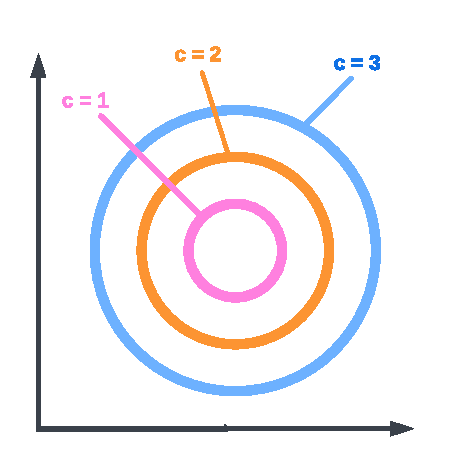
\includegraphics[scale=0.9]{./img/theory/LevelSurfaceSet.pdf}
    \caption{2D example for level surfaces for three different values.}
    \label{fig:level_surface_set}
\end{figure}

Figure \ref{fig:level_surface_set} shows level surfaces for different values of c for a 2-dimensional case. The points on the perimeter of each curve illustrate the set of points sharing the same value, i.e. $f(x_1, x_2) = c$.
\\\\
Recall that a gradient vector is defined as $\nabla f = \left[ \frac{\partial f}{\partial x_1}, \frac{\partial f}{\partial x_2}, ..., \frac{\partial f}{\partial x_d} \right]$.
\\\\
Consider a specific point $\mathbf{x}_0 \in \mathbb{R}^d$. Let us denote the level surface passing through this point by $L_{f(\mathbf{x_0})}$. Let us denote the gradient vector at $\mathbf{x_0}$ by $\nabla f_0$. 
\\\\
Now, consider an arbitrary curve $\mathbf{r}(t) = \left[x_1(t); x_2(t); \ldots, x_d(t)\right]$ (parameterized by a scalar $t$) that passes through $\mathbf{x}_0$, i.e. $\mathbf{r}(t_0) = \mathbf{x_0}$ for some $t_0 \in \mathbb{R}$. Furthermore, 
the curve $\mathbf{r}(t)$ lies within the level surface passing through $\mathbf{x}_0$, i.e. $\mathbf{r}(t) \in L_{f(\mathbf{x_0})}, \,\, \forall t$.  
\\\\
Recall that the tangent to a curve is defined as $\frac{\partial \mathbf{r}}{\partial t}$. 
\\\\
With all that context and notation behind us, now comes the `fun' part. Show that $\nabla f_0$ is orthogonal to the tangent of $\mathbf{r}(t)$ at $t_0$. 
\\\\
Now, please describe in non-technical language what you have just proven. Why might we care about this in the context of deep learning?


\taskbreak

\subsection{Bonus: Relation Gradient - Local Minimum [5 points]}
Consider a (not necessarily convex) differentiable function $g : \mathbb{R}^{n} \rightarrow \mathbb{R}$. $g$ has a local minimum at some $\mathbf{w}^{t}$ if there exists some $\gamma > 0$ such that for all $\mathbf{w} \in \mathbb{R}^{n}$, $\lVert\mathbf{w}^{t} - \mathbf{w}\rVert_{2} < \gamma \Rightarrow g(\mathbf{w}^{t}) \leq g(\mathbf{w})$.

Prove that if $g$ has a local minimum at some $\mathbf{w}^{t}$ then the gradient at $\mathbf{w}^{t} = 0$, and that the converse
is not necessarily true.


\taskbreak

\subsection{Bonus: Relation Gradient - Global Minimum [5 points]}
Prove that if a differentiable function $g : \mathbb{R}^{n} \rightarrow \mathbb{R}$ is convex and the gradient
at some $\mathbf{w}^*$ is 0, then $\mathbf{w}^*$ is the global minimum of $g$.

    
\taskbreak

\subsection{Gradient of the Softmax Function [5 points]}
We will now consider the softmax function $\mathbf{s}(\mathbf{z})$, which takes a vector input $\mathbf{z}$ and outputs a vector whose $i$-th entry $s_i$ is

\begin{equation}
    s_i = \frac{e^{z_{i}}}{\sum_{k} e^{z_{k}}}
\end{equation}

The input vector $\mathbf{z}$ to $\mathbf{s}(\cdot)$ is sometimes called the ``logits'', which just means the unscaled output of previous layers. Derive the gradient of $\mathbf{s}$ with respect to the logits, i.e. derive $\frac{\partial \mathbf{s}}{\partial \mathbf{z}}$. 

